\iffalse
\documentclass[journal,10pt,twocolumn]{article}
\usepackage{graphicx, float}
\usepackage[margin=0.5in]{geometry}
\usepackage{amsmath, bm}
\usepackage{array}
\usepackage{booktabs}
\providecommand{\norm}[1]{\left\lVert#1\right\rVert}
\let\vec\mathbf
\newcommand{\myvec}[1]{\ensuremath{\begin{pmatrix}#1\end{pmatrix}}}
\newcommand{\mydet}[1]{\ensuremath{\begin{vmatrix}#1\end{vmatrix}}}

\title{\textbf{Circle Assignment}}
\author{Alavala Chinnapa Reddy}
\date{September 2022}

\begin{document}

\maketitle
\paragraph{\textit{Problem Statement} -
\fi
In Fig. 		\ref{fig:10/10/2/9}, $XY$ and $EF$ are two parallel tangents to a circle  with centre $\vec{O}$ and another tangent $AB$ with point of contact $\vec{C}$ intersecting $XY$ at $\vec{A}$ and $EF$ at $\vec{B}$. Prove that $\angle{AOB} = 90\degree$.
	\begin{figure}[!h]
		\centering
 \includegraphics[width=\columnwidth]{chapters/10/10/2/9/figs/c.pdf}
		\caption{}
		\label{fig:10/10/2/9}
  	\end{figure}
	\\
\solution
\iffalse
\section*{\large Solution}

\begin{figure}[H]
\centering
\includegraphics[width=1\columnwidth]{figs/c.pdf}
\caption{Tangents from A to circle through P, C and Tangent from B to circle through Q}
\end{figure}
\section*{Solution}
In order to find the intersection points C and P of tangents from A, the origin is  O. The equation of the circle in the new frame is
\begin{equation}
  \boldsymbol{x}^T\boldsymbol{x} = r^2
\end{equation}

\begin{equation}
	\boldsymbol{x} = \vec{A}+\lambda(\vec{m})
\end{equation}
Sub eq2 in eq1
\begin{equation}
	(\vec{A}+\lambda(\vec{m}))^\top(\vec{A}+\lambda(\vec{m}))=r^2
\end{equation}

Simplify eq3
\begin{equation}
	\lambda^{2}\norm{\boldsymbol{m}}^{2}+2\lambda\vec{A}^\top\vec{m}+\norm{\boldsymbol{A}}^{2}=r^{2}
\end{equation}

Solving eq4
\begin{equation}
	\lambda=\frac{-\vec{A}^\top\vec{m}}{\norm{\boldsymbol{m}}^{2}}  
\end{equation}
\begin{equation}
	(\vec{A}^\top\vec{m})^{2}=(\norm{\boldsymbol{A}}-r^{2})(\norm{\boldsymbol{m}}^{2})
\end{equation}
consider
\begin{equation}
	\vec{m}=\myvec{1\\m}
\end{equation}
From eq6
\begin{eqnarray}
	\vec{A}^\top\vec{m}\vec{m}^\top\vec{A}=\norm{\boldsymbol{m}}^{2}(\norm{\boldsymbol{A}}^{2}-r^{2})\\
	\vec{A}^\top\myvec{1&m\\m&m^{2}}\vec{A}=(1+m^{2})(\norm{\boldsymbol{A}}-r^{2})
\end{eqnarray}
consider
\begin{equation}
	\vec{A}=\myvec{a_1\\a_2}=r_1\myvec{\cos{\theta}\\\sin{\theta}}\\
\end{equation}
sub eq10 in eq9
\begin{eqnarray}
	\myvec{a_1&a_2}\myvec{1&m\\m&m^{2}}\myvec{a_1\\a_2}=(1+m^{2})(\norm{\boldsymbol{A}}^{2}-r^{2})\\
	a_1^{2}+2ma_1a_2+m^{2}a_2^{2}=(1+m^{2})(\norm{\boldsymbol{A}}^{2}-r^{2})\\
	m =  \frac{-a_1a_2\pm\sqrt{r^2\norm{\vec{A}}^2-r^4}}{r^2-a_1^2}
\end{eqnarray}
Solving eq13,we get two values $m_1,m_2$.using $\lambda,m_1,m_2$ find two Points intersecting circle at $\vec{P}$ and $\vec{C}$ from eq2
\begin{eqnarray}
	\vec{m_1}=\myvec{1\\m_1}\\
	\vec{m_2}=\myvec{1\\m_2}\\
	\vec{P}=\vec{A}+\lambda\vec{m_1}\\
	\vec{C}=\vec{A}+\lambda\vec{m_2}
\end{eqnarray}
here $\boldsymbol{O}$ is mid point of $\boldsymbol{P}$ and $\boldsymbol{Q}$
\begin{eqnarray}
	\vec{Q}=2(\vec{O})-\vec{P}
	\end{eqnarray}
	assume 
	\begin{equation}
	\vec{D}=\myvec{0&-1\\1&0}
	\end{equation}
\begin{eqnarray}
	\vec{j} = \vec{D}(\vec{P-A})\\
	\vec{k} =\vec{D}(\vec{A-C})\\
	\vec{C}=\myvec{\vec{j^\top}\\\vec{k^\top}}\myvec{\vec{Q} & \vec{A}}\\
	\vec{B}=\myvec{\vec{j^\top}\\\vec{k^\top}}^{-1}\vec{C}
\end{eqnarray}
Using Parallelogram Law Vector Addition
\begin{equation}
	\vec{A-O}=(\vec{P-O})+(\vec{C-O})    
\end{equation}
\begin{eqnarray}
	\vec{B-O}=(\vec{Q-O})+(\vec{C-O})\\
	\vec{B-O}=-(\vec{O-Q})+(\vec{C-O})
\end{eqnarray}
\begin{equation}
	(\vec{A-O})^\top(\vec{B-O})=((\vec{P-O})+(\vec{C-O}))^\top(-(\vec{O-Q})+(\vec{C-O}))
\end{equation}
We Know
\begin{equation}
    \vec{P-O}=\vec{O-Q}
\end{equation}
From eq27 and eq28
\begin{equation}
	(\vec{O-A})^\top(\vec{O-B})=0
\end{equation}
Finally\\
Dot Product of two  Vectors is Zero\\
then,Angle between those two Vectors is  90$^{\circ}$
\begin{equation}
    \angle{\boldsymbol{AOB}}=\boldsymbol{ 90^{\circ}}
\end{equation}
\section*{\large Construction}
{
\setlength\extrarowheight{5pt}
\begin{tabular}{|c|c|c|}
  \hline
  \textbf{Symbol}&\textbf{Value}&\textbf{Description}\\
  \hline
	$r_1$&4&OA \\
  \hline
	$\theta$&120&\\
  \hline
  r&$3$&Radius\\
  \hline
	$\vec{A}$&$r_1\myvec{cos{\theta}\\sin{\theta}}$&Point A\\[5pt]
	\hline
	$\vec{O}$&$\myvec{0\\0}$&Point O\\[5pt]
	\hline
	$\vec{A_O}$&$\vec{A-O}$&$\vec{A}$ when origin shifted to $\vec{O}$\\[5pt]
  \hline
  $m_1,m_2$&evaluate  eq13 &solution of eq13\\[5pt] 
  \hline
	$\vec{C}$&$\vec{A}+\lambda\vec{m_2}$&Point C\\[5pt]
  \hline
	$\vec{P}$&$\vec{A}+\lambda\vec{m_1}$&Point P\\[5pt]
	\hline
	$\vec{Q}$&2$(\vec{O})-\vec{P}$& Point Q\\
	\hline
	$\vec{B}$&$\myvec{j^\top\\k^\top}\vec{c}$&Point B\\[5pt]
	\hline
\end{tabular}
}
\end{document}
\fi
